\documentclass[11pt]{article}
\usepackage{fullpage}
\usepackage{graphicx}
\usepackage{natbib}
\usepackage{hyperref}

\begin{document}
\title{Radio Skillz: Digital Lab 2}

\maketitle

\section*{Prerequisites}

\begin{itemize}
\item Synchronous and Asynchronous Logic
\item Processor Architectures
\item Convolution Theorem
\item Digital Down Conversion
\end{itemize}

\section*{Materials}

\begin{itemize}
\item ROACH board
\item quad-ADC board
\item 200 MHz clock source
\item 0-400 MHz tone generator
\item noise generator
\item various low-pass and band-pass filters
\end{itemize}

\section*{Some Thoughts}

\subsection*{Simulink}

\subsubsection*{Setting up a VNC Session}

From any *nix computer:
\begin{verbatim}
ssh -Y gbower@otto.eecs.berkeley.edu
$ ssh username@host.computer.edu
    (enter password)
$ vncserver
    (write down XX of "desktop is host.computer.edu:XX)
$ exit
\end{verbatim}
This will set up a VNC session for you to log into in the future.  Remember
your session number (XX).

When you are done with your session, it would be neighborly of you to free up the computer resources associated with your vnc session:
\begin{verbatim}
$ ssh username@host.computer.edu
$ vncserver -kill :XX
    (where XX is your VNC session from above)
$ exit
\end{verbatim}
Thanks!

\subsubsection*{Accessing Your VNC Session}

From any *nix computer:
\begin{verbatim}
$ vncviewer -via username@host.computer.edu localhost:XX
    (ssh password)
    (vnc password)
\end{verbatim}

All future commands are to be typed inside your VNC session.

%\subsection{About Simulink on Linux}
%
%The machine you are logged into is running a Linux desktop.
%It behaves somewhat differently than other desktop environments you may be
%used to.  Because Simulink sometimes opens windows that are larger than
%the size of the desktop, it may be useful to know that you can move these
%windows around by right-clicking, selecting "Move", and then dragging the window around.

\subsubsection*{Starting Matlab/Simulink}

%Make sure there is a file "startup.m" in your directory.  If it does not
%exist, copy it there from /opt/casper/startup.m.  This file is required to
%automatically load some signal processing libraries when you start up
%the design tools.
To start Matlab/Simulink, type:

\begin{verbatim}
$ cd ~/mlib_devel
$ ./simmy_hitz
\end{verbatim}

This program is a script that sets up the licenses for all the tools we'll be
using, and then executes the program ``matlab''.  All further commands will be in
the matlab window, unless we say otherwise.

\section{Introduction to Simulink and ROACH: Tweaking the ADC Sampler}

In this lab, we're going to cut corners so that you can get done faster. 
If you want a more thorough introduction to Simulink and FPGA programming, we have a nice
tutorial\footnote{\url{http://casper.berkeley.edu/astrobaki/index.php/CasperTutorial01}}
that will run you through the basics (skip section 8, which you don't need).
A few details from that tutorial are different for the setup in our lab. 
The ROACH we use has an "lx110t" FPGA, (not "sx95t"), so set the {\it XSG Core Config} block accordingly.
You'll also need to scp you *.bof file from our compile server over to a local machine before
sending it to the roach.  You'll also have to use the correct IP address for the ROACH.

\subsection{Reviewing the ADC Sampler}

\begin{figure}\centering
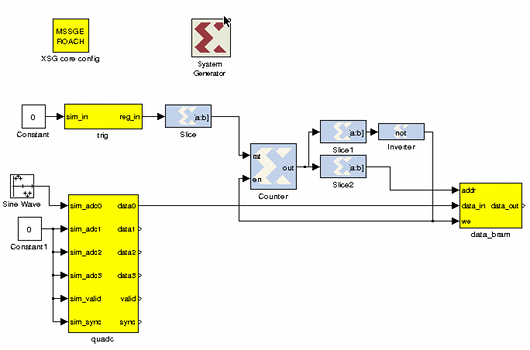
\includegraphics[width=4in]{digital_lab_2_plots/adc_capture.png}
\end{figure}

\begin{itemize}
\item open simulink:
\begin{verbatim}
>> simulink
\end{verbatim}
\item open the file \url{~/aparsons/adcsampler.mdl}
\item save this mdl to \url{~/yourname/adcsampler.mdl}
\item poke around to understand the idea:
\begin{itemize}
\item in {\tt XSG core config}: compile for = ROACH:ls110t, Clock Rate (MHz) = 200
\item in {\tt trig}: I/O direction = from processor, Data Type = unsigned
\item in {\tt trig\_slice}: offset of bottom bit = 0
\item in {\tt counter}: output type = unsigned, number of bits = 14 
\item in {\tt addr\_slice}: width of slice = 13, offset of bottom bit = 0
\item in {\tt stop\_slice}: boolean output = true, offset of top bit = 0
\item in {\tt data\_bram}: data type = signed, address width = 13, data binary point = 7
\end{itemize}
\item you can use Edit$\to$Update Diagram to display ports.
Although this will complain
if your design isn't complete (i.e. if there are errors), it will tell you the data
type of each wire of a working design.  This can really help you follow how your
design works and catch bugs before compiling.  If you change your design, hit Ctrl-D
to update the labels.
\item interpreting data types: Fix8\_7 means (signed) fixed point, 8 bits, 7 bits after the binary point.
\item another useful tool: right-click$\to$Look Under Mask
\end{itemize}

\subsection{Tweaking the ADC Sampler: Applying a Summing Filter}

\begin{itemize}
\item modify (but save to a new file) your design to capture ADC samples, so that two adjacent input time samples are summed
to produce each output sample.  Stated more precisely, produce the output $S$ such that:
\begin{equation}
S_i = X_{i-1} + X_{i-2}
\end{equation}
where $X_i$ are input samples.  Note that the latency of your summing filter is unimportant.
You can find blocks in the Simulink window under the Xilinx Blockset$\to$Index.
\item before you compile, you can simulate your design to ensure everything is working.  Take a look at
the Scope block in the standard Simulink library. You'll have to use Gateway Outs (from the Xilinx Blockset)
to convert from fixed point data to doubles, which the Scope needs as inputs for plotting. 
\item compile your design (this will take 5-10 minutes):
\begin{verbatim}
>> bee_xps
\end{verbatim}
The bof file shows up in <design name>/bit\_files
\end{itemize}

Before programming the ROACH with this design:
\begin{itemize}
\item Can you predict a priori what frequency response this time-domain 
summing filter will produce (hint: it {\it is} an analytic function)?
\item inject the same noise source into you new design (and capture data) and the old adcsampler (already compiled in the aparsons directory).  
\item Use your measured power spectra to isolate the inherent response of your summing filter
\item Overlay on your measured filter response the filter response you predicted
\item Is your prediction accurate to within the noise of your measurements? It better be!
\end{itemize}


%A picture of a working design has been included as a reference should you get stuck.  However, you'll
%have to figure out the block parameters for yourself.  One thing to be sure of: make sure the {\bf XSG Core Config}
%block in your design is set for "User IP Clock Source" = "adc0\_clk".  This uses the ADC sample clock 
%to clock the FPGA, so everything marches through the FPGA at the rate that samples arrive.

\section{Using the Down-Converter Design}

\begin{itemize}
\item open the file \url{~/aparsons/downconverter.mdl}
\item by reading the design, figure out how to set a mixing frequency and capture data.  Poke around to get a feel for how these designs work (you'll have to modify this design reasonably substantially next lab).
\item describe in words how the design works, and how to use it.
\item run the design manually, with a known input signal, to verify that you get a down-coverted tone out.
\end{itemize}

\section{Automating Data Collection to Characterize Filter}

\begin{itemize}
\item write a program that automatically sets the mixing tone to various frequencies and captures the relevant data.
\item run the program with a fixed analog input tone, trying enough frequencies to be able to characterize the
digital filter.  You might want to file the data captures under meaningful names for later use.
\item write another program that uses these various data captures to plot the digital filter shape.  Does it
agree with predictions?  Again, it better!
\end{itemize}

\end{document}
